\documentclass{source/Experiment}

\major{信息工程}
\name{姚桂涛}
\title{}
\stuid{3190105597}
\college{信息与电子工程学院}
\date{\today}
\lab{}
\course{}
\instructor{}
\grades{}
\expname{聚丙烯熔融指数预测}
\exptype{}
\partner{}

\begin{document}
    \begin{center}
        \vspace{0.5cm}
        \bfseries\Large{软件技术基础大作业——聚丙烯熔融指数预测}
    \end{center}

    \section{问题背景}
        \subsection{聚丙烯熔融指数预测}
        数据来源:聚丙烯生产过程熔融指数数据,共 150 组时序数据,见 excel 表格。 问题描述:聚丙烯生产过程中的熔融指数是一个重要质量控制指标(excel 表格中的 变 量 y),决定了所生产产品的牌号与价格,但是难以在线测量,从而导致生产质量的控制品 质大大降低。因此,采用生产中与该质量控制指标相关的可直接测量的操作变量(excel 表 格中的变量 x,共 9 个),来在线预测该质量控制指标,从而提高生产质量控制品质。

    \section{实验任务}
    
        根据所给的数据集,建立一个模型,从而能够预测聚丙烯熔指指数指标。

    \section{设计过程}
        初步拿到数据,发现有9个输入变量,1个输出变量。题目要求是希望能够在线预测质量控制指标,从而提高生产质量控制品质。所以初步判断这是一个多元的回归问题。
        根据所学到的知识以及所查阅的资料,我首先的想法是通过使用sklearn进行数据集训练与模型建立。同时利用pandas库和numpy库对数据进行操作。
        \subsection{数据处理}
            题目所提供数据为xls格式,如下图所示:
            \begin{figure}[H]
                \centering
                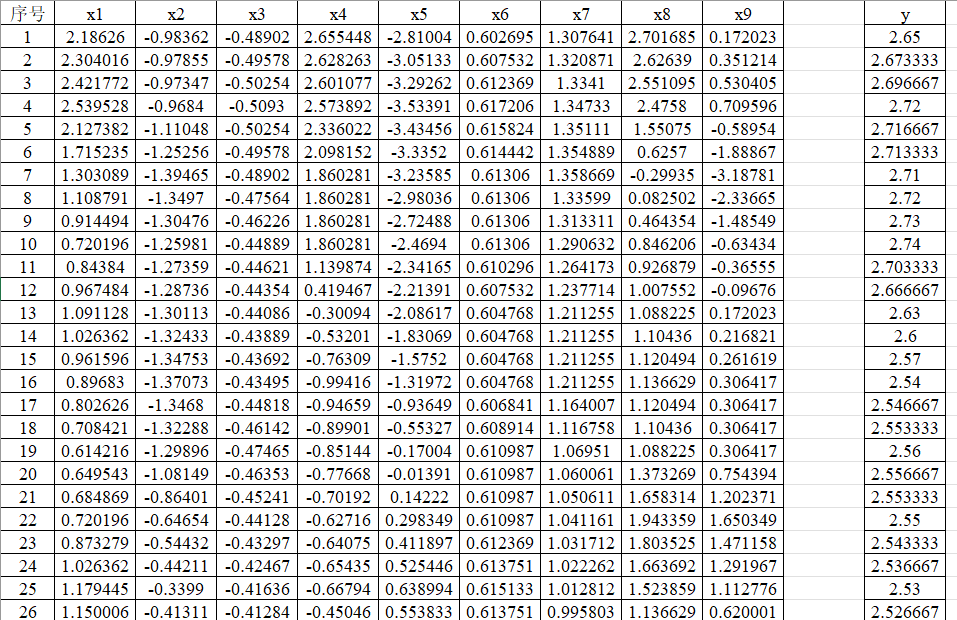
\includegraphics[width = 0.8\textwidth]{原始数据}
                \caption{原始数据}
            \end{figure}
            为了方便python操作,将数据第一列删除,'y'列与左边靠拢,并保存为csv格式。

            调用corr函数,查看各个输入变量x与y之间的相关系数,并通过seaborn库绘制可视化相关程度的热图如下:
            \begin{figure}[H]
                \centering
                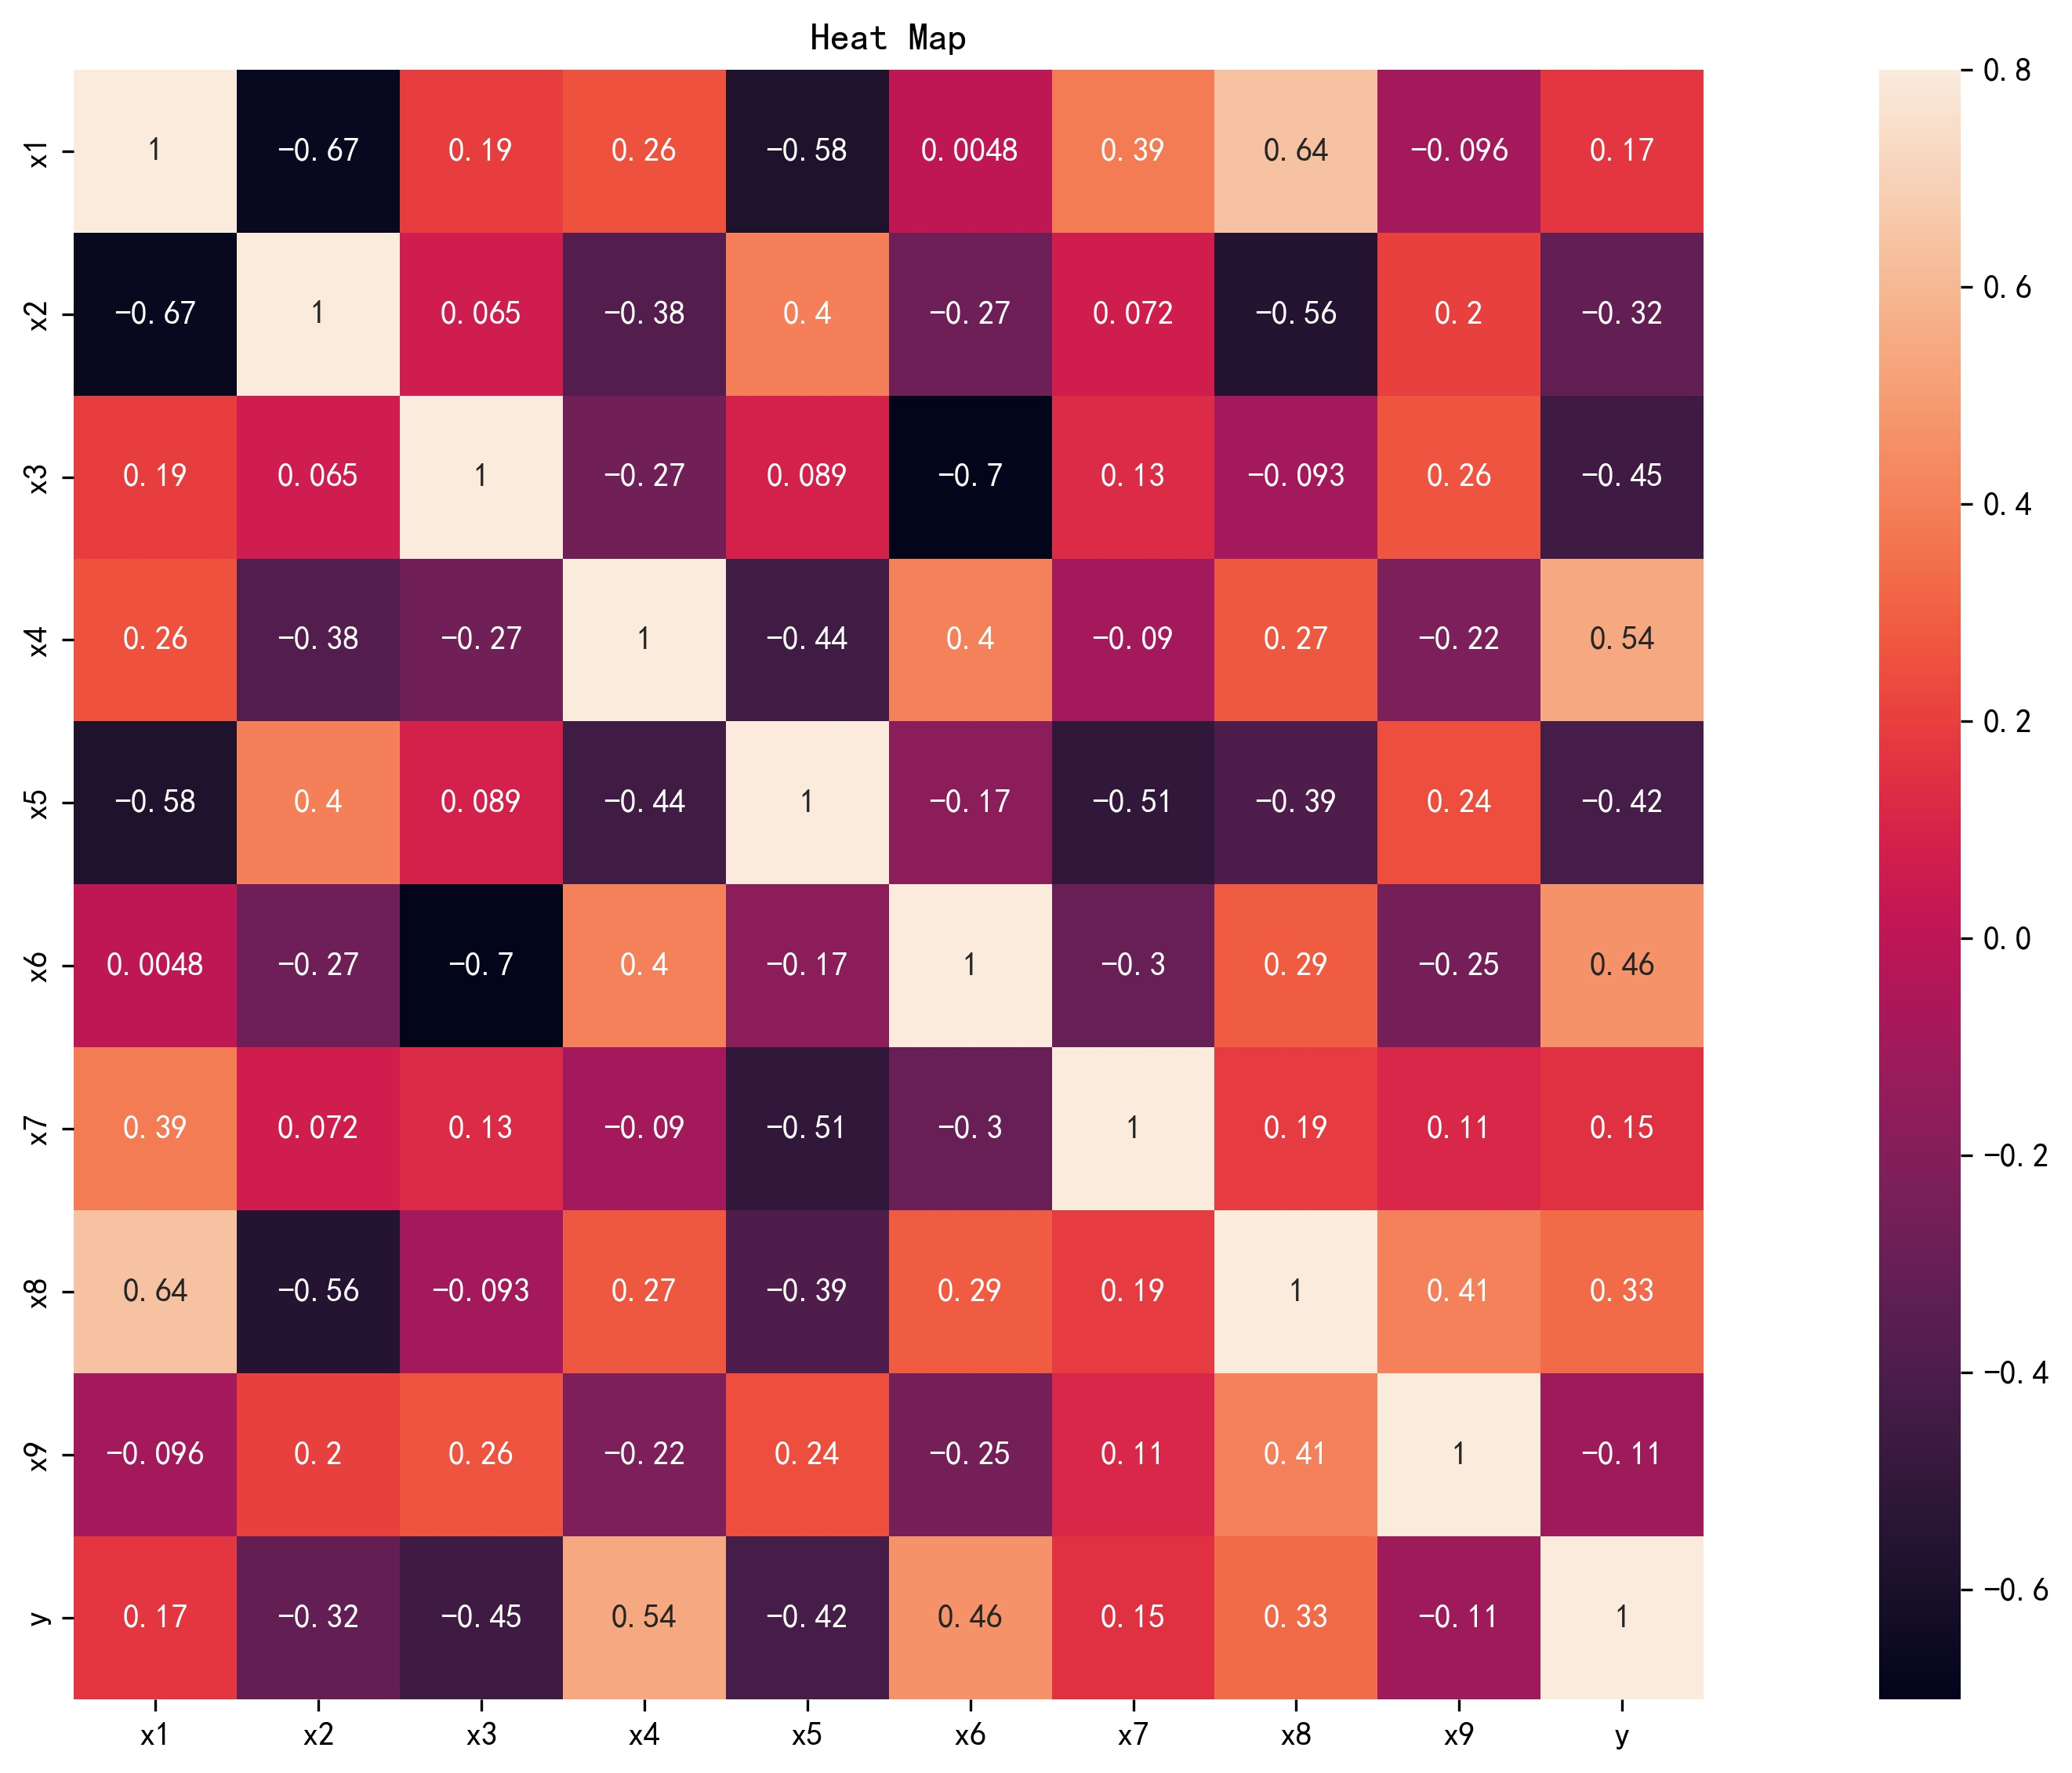
\includegraphics[width = 0.65\textwidth]{HeatMap}
                \caption{输入输出相关性}
            \end{figure}
            可以看出输入变量x1-x9与输出变量y的相关性普遍比较低,最高的也只是x3,x4,x5,x6这几个变量。

            于是我决定先选用x3,x4,x5,x6这四个输入作为训练输入,由于无法确定该问题是线性回归还是非线性回归,于是我首先尝试了线性回归。

            先利用train\_test\_split函数将数据集划分为训练集和测试集
            \begin{lstlisting}[language=Python]
X_train2, X_test2, Y_train2, Y_test2 = train_test_split(X_Poly, y, train_size=0.80, random_state=1)
            \end{lstlisting}

            这里将150个数据随机分成120个训练集X\_train1,Y\_train1和30个测试集X\_test1,Y\_test1。

            随后利用scikit-learn框架中的LinearRegression模型中,使用fit函数进行训练,最后得到对应的线性回归方程。
            得到模型结剧a,回归系数b。
            \begin{lstlisting}[language=Python]
model = LinearRegression()
model.fit(X_train, Y_train)
print("截距:",LinearR.intercept_)
print("系数:",LinearR.coef_)
            \end{lstlisting}
            得到结果如下:
            \begin{lstlisting}[language=Python]
截距:2.4513199017988554
系数:[-0.0391533  -0.03018913 -0.03880207  0.05311798 -0.00549697  0.01419835
0.05236998  0.01524657  0.0052771 ]
y = -0.0391533*x1 + -0.03018913*x2 + -0.03880207*x3 + 0.05311798*x4 + -0.00549697*x5 + 0.01419835*x6 + 0.05236998*x7 + 0.01524657*x8 + 0.0052771*x9
            \end{lstlisting}
            在得到结果后,通过模型的predict函数对数据进行了预测,并且使用模型的mean\_squared\_error函数和R\^2检测r2\_score函数进行了模型评分。
            \begin{lstlisting}[language=Python]
Y_pred1 = LinearR.predict(X_test1)
# 平均误差相对于样本真实值均值偏差
print("mse相对于测试值平均值的偏差:", np.sqrt(MSE(Y_test1, Y_pred1))/Y_test1.mean())
# R^2检测
print("r2检测:", r2_score(y_true=Y_test1, y_pred=Y_pred1))
            \end{lstlisting}
            得到结果如下:
            MSE相对于测试值平均值的偏差: 0.03954403176473497
            
            $\rm R^2$检测结果为:0.2770634859513812

            \begin{figure}[H]
                \centering
                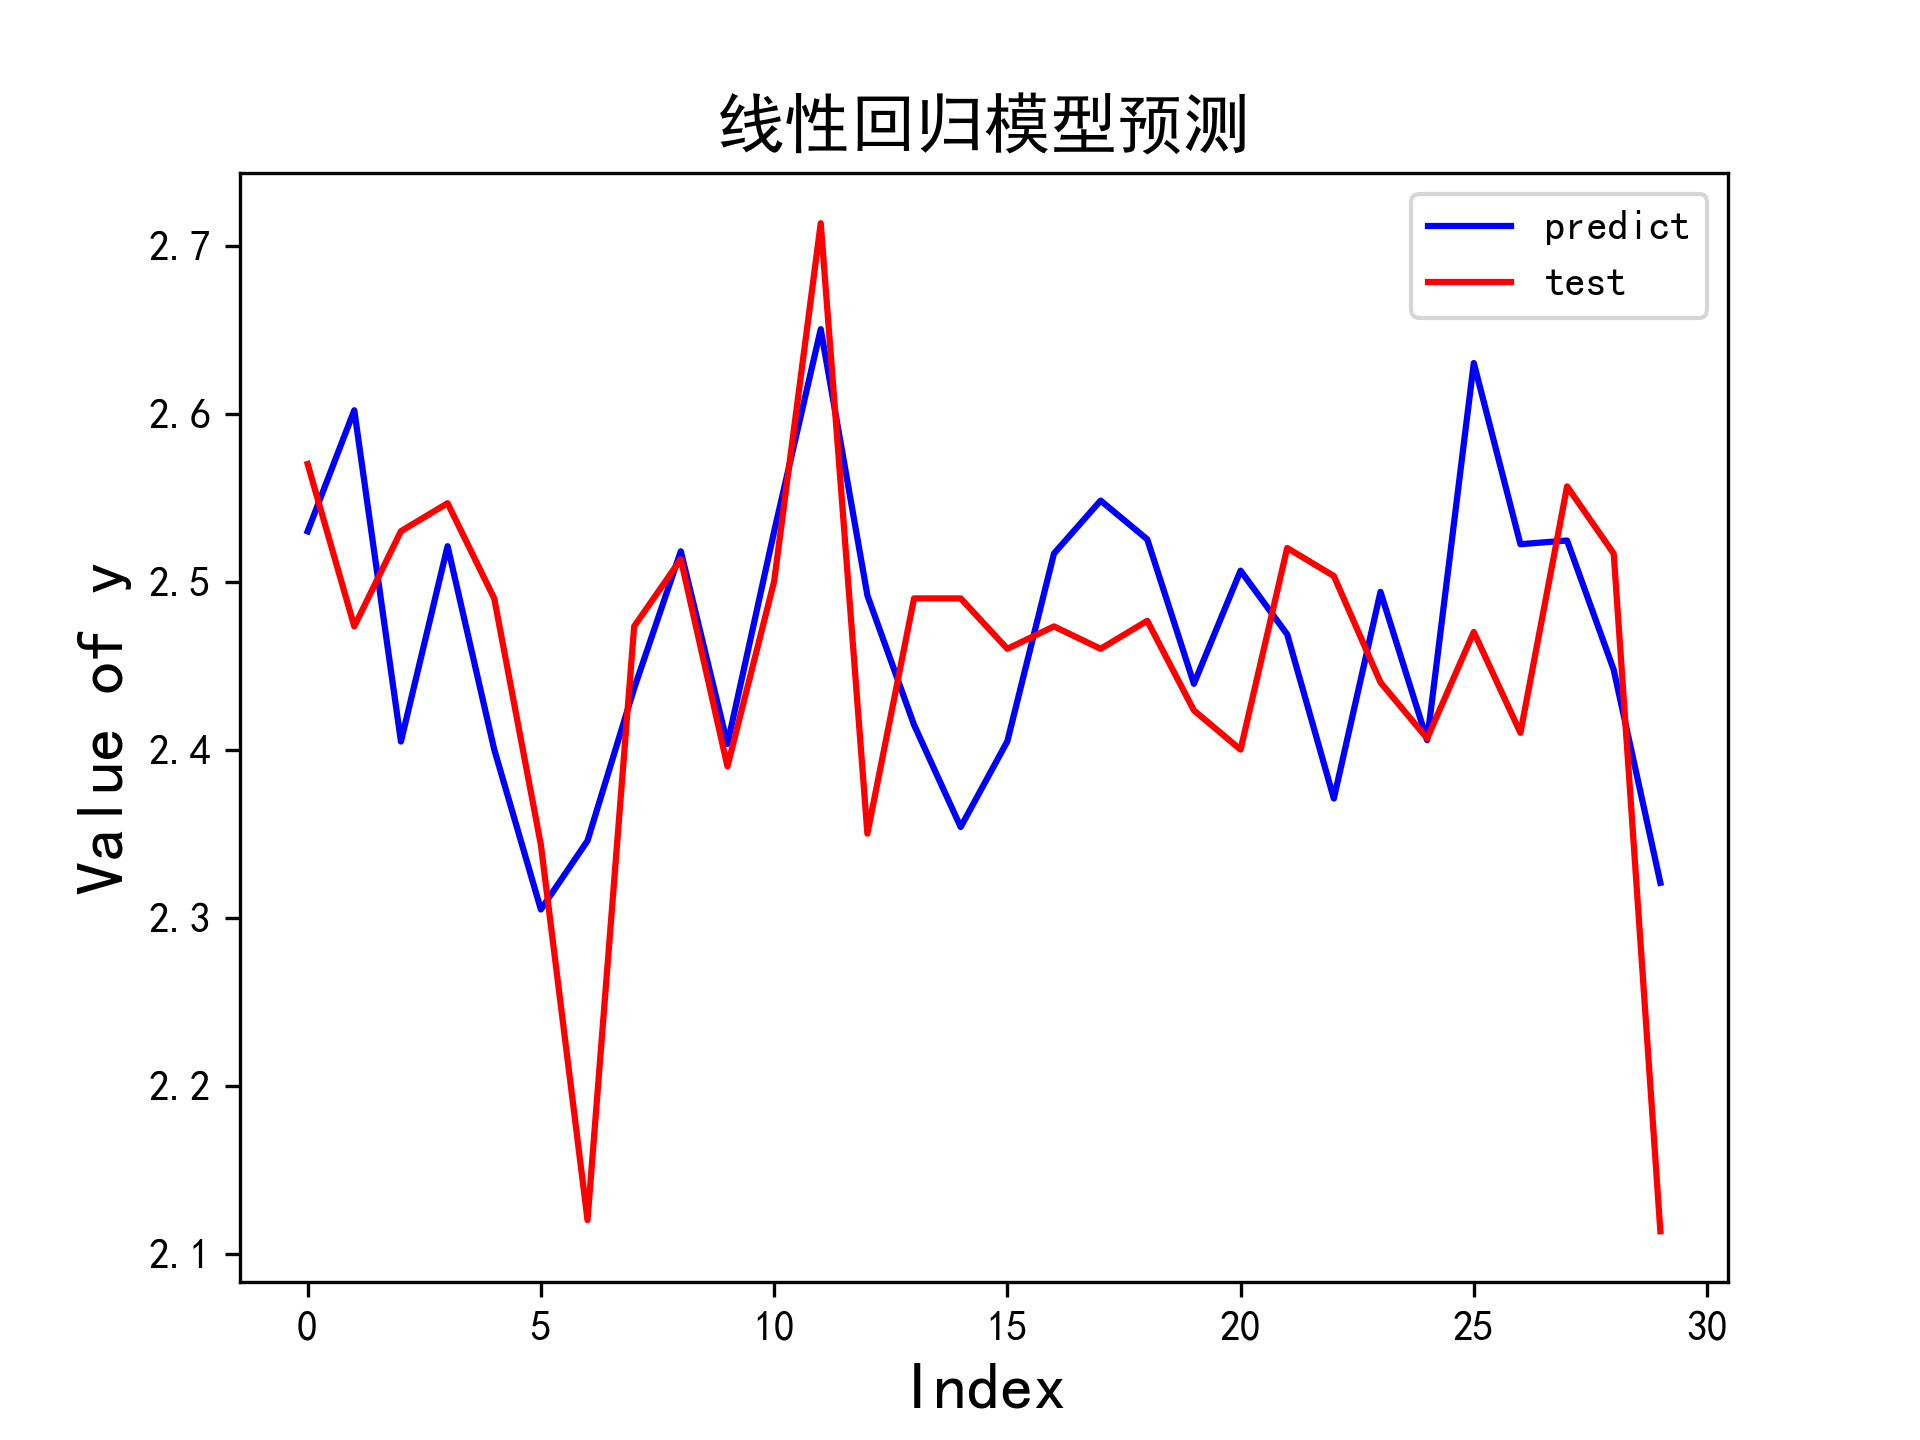
\includegraphics[width = 0.6\textwidth]{LinearR}
                \caption{预测和测试输出比较}
            \end{figure}
            
            从结果可以看出,训练得到的线性模型性能并不长非常的理想。于是我又尝试用非线性回归模型进行预测。此处我先尝试了用二次多项式回归模型。

            首先需要给原来的一次特征x1~x9添加二次特征,此处用到了sklearn库里的PolynomialFeatures函数。并利用fit\_transfrom对特征进行预处理(标准化、归一化等)。
            \begin{lstlisting}[language=Python]
PolyF = PolynomialFeatures(degree=2, interaction_only=False, include_bias=False)
X_Poly = PolyF.fit_transform(x)
            \end{lstlisting}
            然后同样对数据集进行分割,并使用LinearRegression模型进行训练,得到结果如下:
            \begin{lstlisting}[language=Python]
X_train2, X_test2, Y_train2, Y_test2 = train_test_split(
    X_Poly, y, train_size=0.80, random_state=1)
LinearR2 = LinearRegression().fit(X_train2, Y_train2)
print("截距:",LinearR2.intercept_)
print("系数:",LinearR2.coef_)
            \end{lstlisting}
            \begin{lstlisting}
截距: 2.573018518031015
系数: [ 0.04056469 -0.16426964 -0.46139441 -0.00801811  0.32999633 -0.64890163
 -0.43351057 -0.13721673  0.09905394 -0.0620823  -0.00969554  0.16997955
  0.0299021  -0.00500646  0.09598441  0.02758844 -0.02453116 -0.00945735
  0.00353089  0.77368019 -0.00336322  0.21904659  0.55840549  0.04788288
  0.05353425 -0.01597955 -0.06088869  0.0826872  -0.82603222 -0.19639567
 -0.79049372 -0.08128735  0.134005   -0.00179539 -0.00387439  0.0046151
 -0.03845884  0.10717514 -0.0532185   0.03376222 -0.28864873 -0.19171991
  0.01174273 -0.01913421  0.00768826  0.46659538 -0.13289949  0.09817754
 -0.01131589 -0.02820713  0.00396911  0.01439626  0.07039836 -0.04216297]
\end{lstlisting}
            按照同样的方法进行预测并评估模型性能:
            \begin{lstlisting}[language=Python]
Y_pred2 = LinearR2.predict(X_test2)
# 平均误差相对于样本真实值均值偏差
print("mse相对于测试值平均值的偏差:", np.sqrt(MSE(Y_test2, Y_pred2))/Y_test2.mean())
# R^2检测
print("r2检测:", r2_score(y_true=Y_test2, y_pred=Y_pred2))
            \end{lstlisting}
            结果如下:

            mse相对于测试值平均值的偏差: 0.011169084653174191

            r2检测: 0.9423268817732235

            \begin{figure}[H]
                \centering
                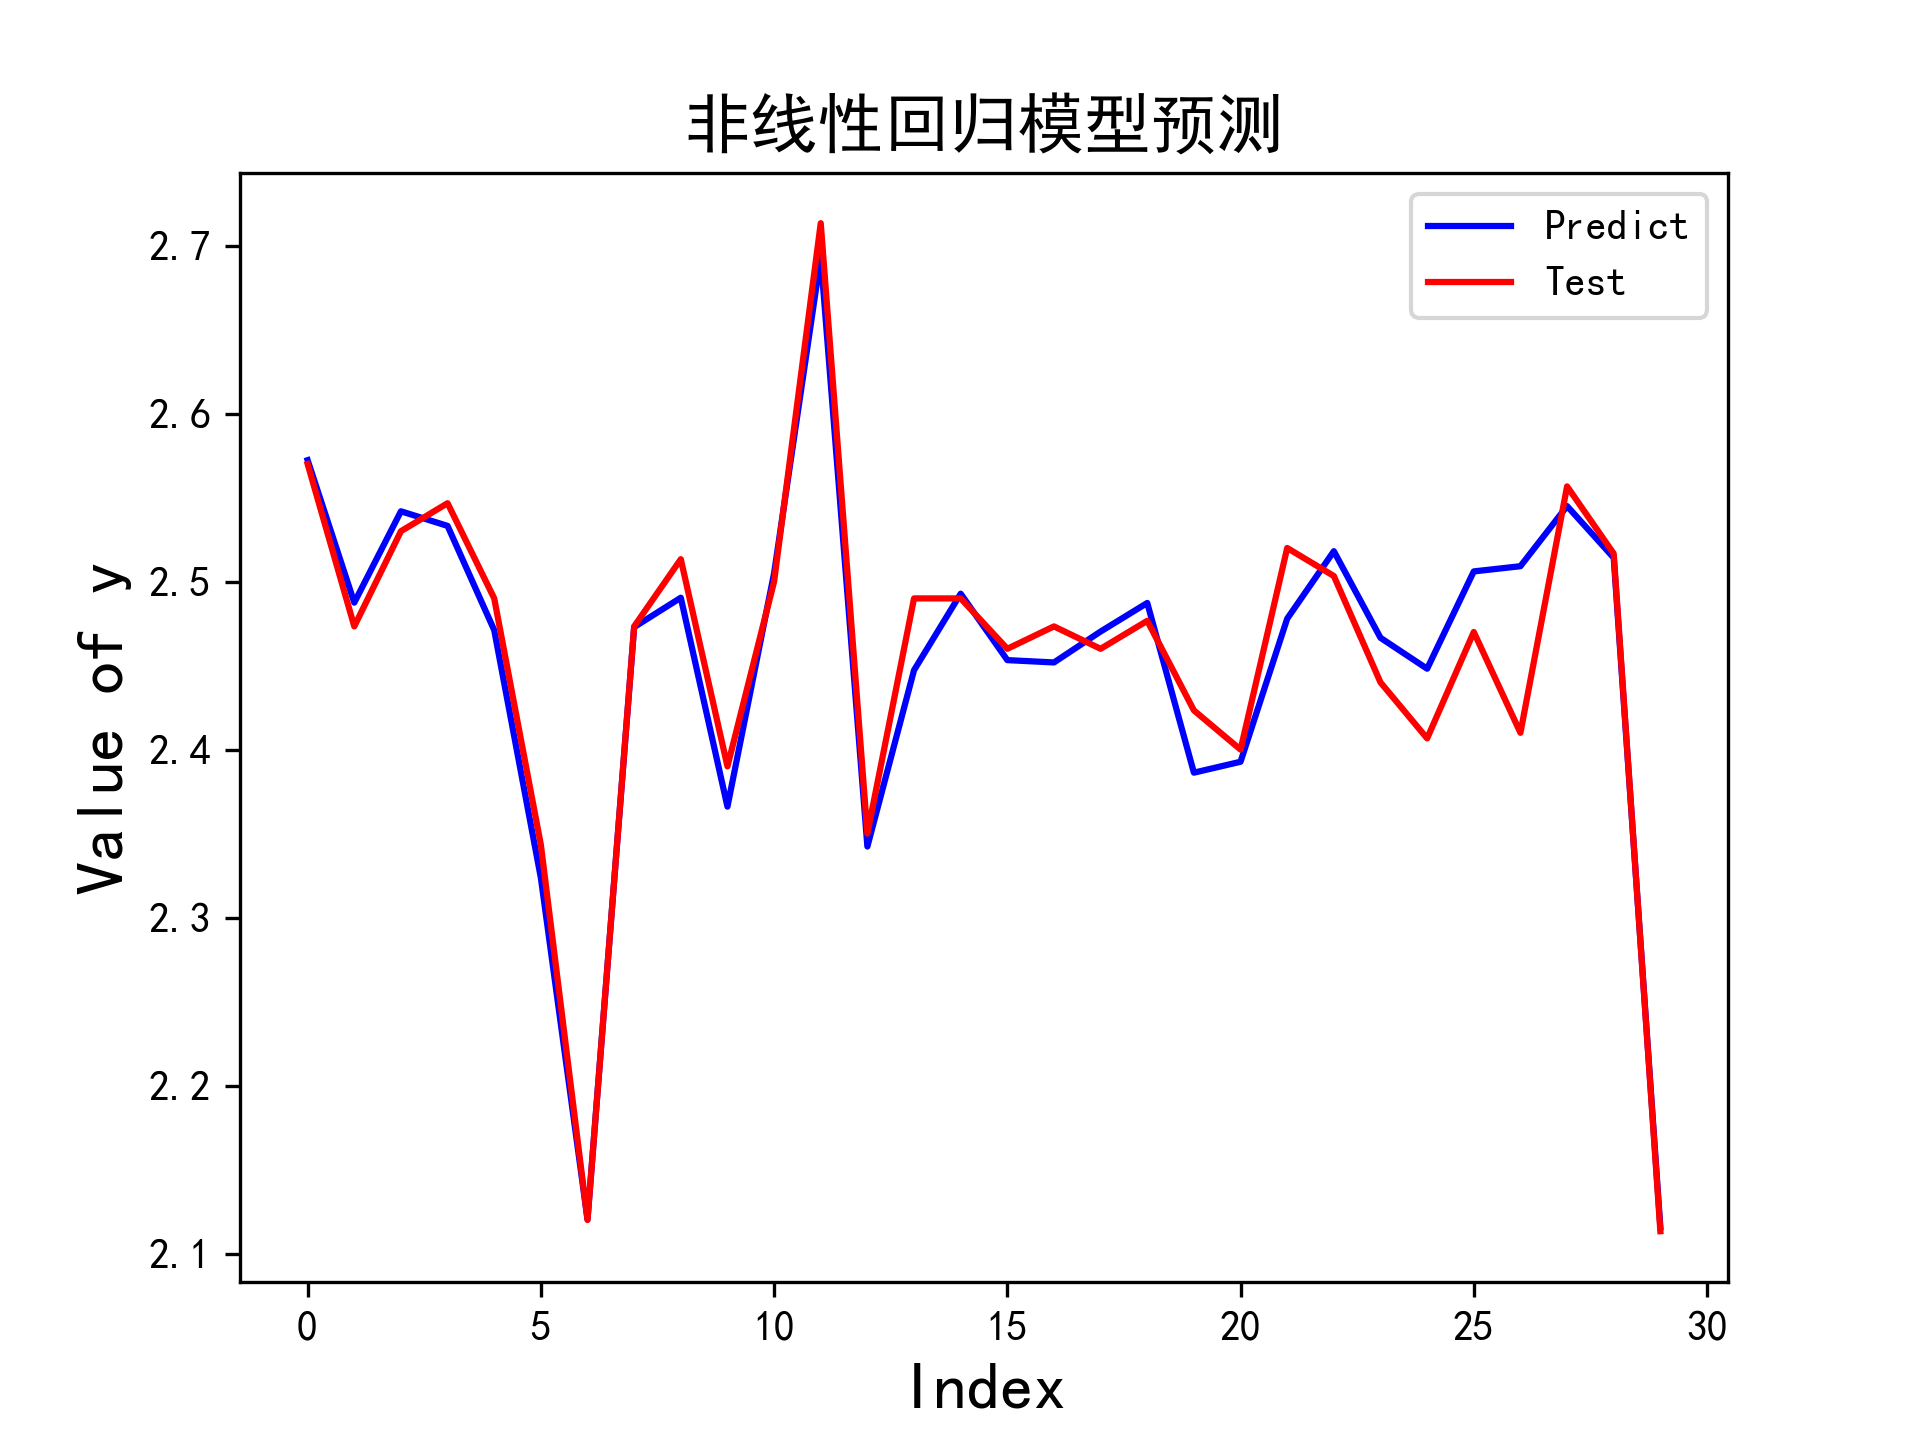
\includegraphics[width = 0.6\textwidth]{LinearR2}
                \caption{预测和测试输出比较}
            \end{figure}

            可以看到,利用二次多项式回归模型的性能达到了比较好的水平。
    \section{实验代码}
        \lstinputlisting[
                        language  =   Python
            ]{PolynomialFeatures.py}
    \section{实验心得与体会}
        \begin{enumerate}
            \item 本次实验最大的困难其实是如何将上课所讲的知识点实现出来。为此我查阅了大量的资料。因为之前只用过matlab,所以一开始我想从matlab入手解决问题,但是当我查阅资料时发现大部分类似的问题解决方案都是用python语言解决的。所以我首花了一个多小时时间配置pyhton环境,最终我选择了利用Anaconda,因为它方便管理和导入各种库。
            \item 在确定语言为python后,我对问题进行了初步的分析,决定从建立回归模型角度去解决问题,由此开始查阅资料学习python相关的可以进行回归分析训练的库。最后决定使用scikit-learn这一个库进行核心的模型建立训练,同时使用pandas和mumpy库处理数据,以及seaborn库分析结果和matplotlib库绘制图像。
            \item 本次大作业我最大的收获首先是对于课堂上所学的机器学习的内容有了更深刻的理解,对于许多概念进行了实现,不再是概念了解。其次是对于pyhton这门语言有了初步的掌握和理解。
        \end{enumerate}
\end{document}